\begin{frame}
  \frametitle{Memoria}
  \begin{itemize}
	  \item La organización y administración de la \textit{memoria RAM} es uno de los factores más importantes en el diseño de un SO
	  \item Los programas y datos deben residir en ella para:
	  \begin{itemize}
	  	\item Poder ejecutar
	  	\item Referenciarlos directamente
	  \end{itemize}
  \end{itemize}
\end{frame}

\begin{frame}
  \frametitle{Memoria (cont.)}
  \begin{itemize}
	  \item La parte del SO que administra esta memoria se llama ``\textit{administrador de la memoria}'':
	  \begin{itemize}
	  	\item Lleva un registro de las partes de la memoria que se están utilizando y de aquellas que no
	  	\item Asigna espacio en memoria a los procesos cuando estos la necesitan
	  	\item Libera espacio de momoria asignada a procesos que han terminado
	  \end{itemize}
	  \item Se espera que el SO haga uso eficiente de esta memoria con el fin de alojar el mayor número de procesos $\rightarrow$ repercute en la \emph{multiprogramación}
  \end{itemize}
\end{frame}

\begin{frame}
  \frametitle{Direccionamiento}
  \begin{itemize}
	  \item \textbf{Dirección Lógica}:
	  \begin{itemize}
	  	\item Es una dirección que enmascara o abstrae una dirección física
	  	\item Referencia a una localidad en memoria
	  	\item Se la debe traducir a una dirección física
	  \end{itemize}
	  \item \textbf{Dirección Física}:
	  \begin{itemize}
	  	\item Es la dirección real. Es con la que se accede efectivamente a memoria
	  	\item Representa la dirección absoluta en memoria principal
	  \end{itemize}
	  \item La CPU trabaja con direcciones lógicas. Para acceder a la memoria se deben transformar en direcciones físicas
	  \item El mapeo entre direcciones virtuales y físicas se realiza mediante \emph{hardware} $\rightarrow$ \textbf{MMU} (Memory Management Unit)
  \end{itemize}
\end{frame}

\begin{frame}
  \frametitle{Traduccion \textbf{MMU}}
  \begin{figure}
    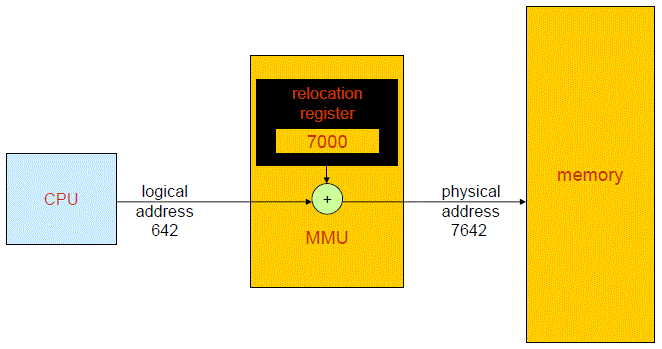
\includegraphics[scale=0.4]{images/mmu.png}
  \end{figure}
\end{frame}

\begin{frame}
  \frametitle{Asignación de memoria}
  \begin{itemize}
	  \item \textbf{Particiones Fijas}:
	  \begin{itemize}
	  	\item La memoria se divide en particiones o regiones de tamaño fijo $\rightarrow$ tamaños iguales o diferentes
	  	\item Alojan un único proceso
	  	\item Cada proceso se coloca en alguna partición de acuerdo a algún criterio:
	  	\begin{itemize}
	  		\item \textbf{First Fit}
	  		\item \textbf{Best Fit}
	  		\item \textbf{Worst Fit}
	  		\item \textbf{Next Fit}
	  	\end{itemize}
	  \end{itemize}
	  \item \textbf{Particiones Dinámicas}:
	  \begin{itemize}
	  	\item Las particiones varían en tamaño y número
	  	\item Alojan un proceso cada una
	  	\item Cada partición se genera en forma dinámica del tamaño justo que necesita el proceso
	  \end{itemize}

	  \pause
	  \hspace{35pt} \textcolor{orange}{¿Qué problemas se generan en cada caso?}
  \end{itemize}
\end{frame}

\begin{frame}
  \frametitle{\textbf{Fragmentación}}
  \begin{itemize}
  	  \item La fragmentación se produce cuando una localidad de memoria no puede ser utilizada por no encontrarse en forma contigua
	  \item \textbf{Fragmentación Interna}:
	  \begin{itemize}
	  	\item Se produce en el esquema de particiones fijas, por ejemplo
	  	\item Es interna a la localidad asignada
	  	\item Es la porción de la localidad que queda sin utilizar
	  \end{itemize}
	  \item \textbf{Fragmentación Externa}:
	  \begin{itemize}
	  	\item Se produce en el esquema de particiones dinámicas, por ejemplo
	  	\item son huecos que van quedando en la memoria a medida que los procesos finalizan
	  	\item Al no encontrarse en forma contigua puede darse el caso de que tengamos memoria libre para alocar un proceso, pero que no la podamos utilizar
	  	\item Solución $\rightarrow$ \emph{compactación} $\rightarrow$ muy costosa
	  \end{itemize}
  \end{itemize}
\end{frame}

\begin{frame}
  \frametitle{\textbf{Paginación}}
  \begin{itemize}
  	  \item La memoria se divide en porciones de igual tamaño llamadas \emph{\emph{marco}}
	  \item El espacio de direcciones de los procesos se divide en porciones de igual tamaño denominadas \textbf{páginas}
	  \item Tamaño página = tamaño \emph{marco} = 512 bytes (generalmente)
	  \item El SO mantiene una tabla de páginas para cada proceso, la cual contiene el \emph{marco} donde se encuentra cada página
	  \item La paginación bajo demanda es una técnica eficiente de manejar esta estrategia $\rightarrow$ \emph{Thrashing}
  \end{itemize}
\end{frame}

\begin{frame}
  \frametitle{Paginación - \textbf{Direccionamiento}}
  \begin{figure}
    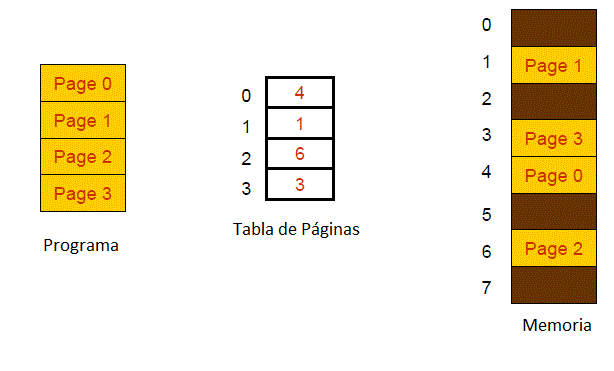
\includegraphics[scale=0.5]{images/pagination1.png}
  \end{figure}
\end{frame}

\begin{frame}
  \frametitle{Paginación - \textbf{Direccionamiento} (cont.)}
  \begin{itemize}
  	  \item Un proceso en ejecución hace referencia a una dirección virtual $\rightarrow$ \emph{v = (p,d)}
	  \item El SO busca la página \emph{p} en la \emph{tabla de páginas} del proceso y determina en que \emph{marco} se encuentra
	  \item La dirección de almacenamiento real se forma por la concatenación de la resolución de \emph{p} (dirección inicio del marco que aloca la página) y \emph{d}, donde \emph{p} es el número de página y \emph{d} es el desplazamiento
  \end{itemize}
\end{frame}

\begin{frame}
  \frametitle{Paginación - Ejemplo}
  \begin{itemize}
  	  \item Memoria administrada por sistema de paginacion
	  \item Tamaño de página $\rightarrow$ 515 Bytes
	  \item Cada dirección de memoria referencia a 1 Byte
	  \item Los \emph{marco} en memoria principal se encuentran desde la dirección física 0
	  \item Tenemos un proceso con un tamaño de 2000 Bytes y con la siguiente tabla de páginas
  \end{itemize}
\end{frame}

\begin{frame}
  \frametitle{Paginación - Ejemplo (cont.)}
  \begin{figure}
    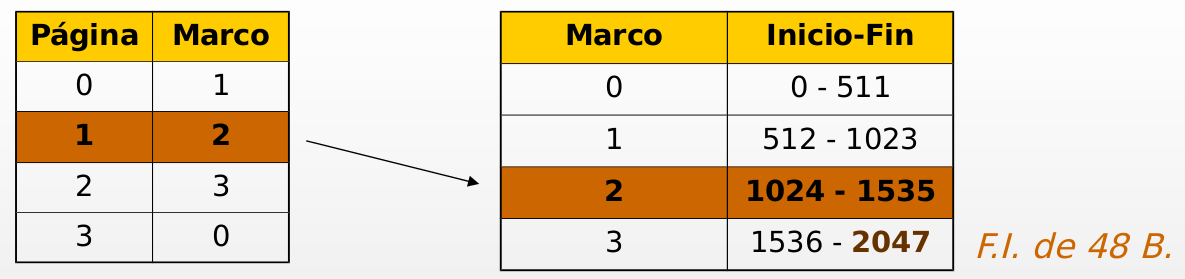
\includegraphics[scale=0.2]{images/pagination2.png}
  \end{figure}
  \begin{itemize}
  	\item Si tenemos una dirección \textbf{lógica}, por ejemplo 580:
  	\begin{itemize}
  		\item Para averiguar el número de página hacemos 580 div 512 = 1. Luego esta dirección corresponde a la página 1 que se encuentra en el \emph{marco} 2
  		\item Para averiguar el desplazamiento hacemos 580 mod 512 = 68
  		\item La dirección física es 1024 + 68 = 1092
  	\end{itemize}
  \end{itemize}
\end{frame}

\begin{frame}
  \frametitle{Paginación - Ejemplo (cont.)}
  \begin{figure}
    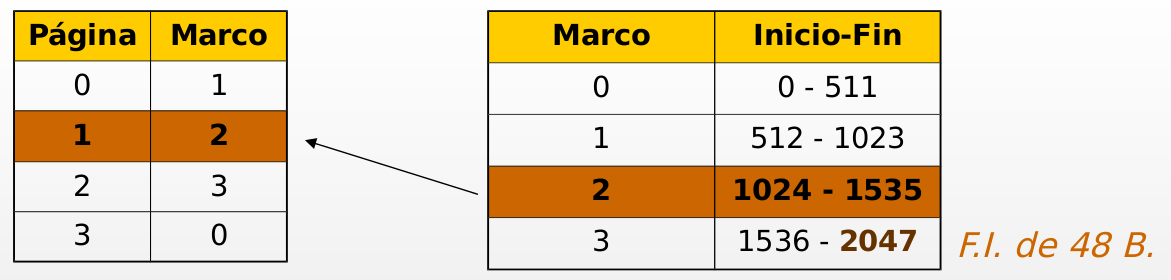
\includegraphics[scale=0.2]{images/pagination3.png}
  \end{figure}
  \begin{itemize}
  	\item Si tenemos una dirección \textbf{física}, por ejemplo 1092:
  	\begin{itemize}
  		\item Para averiguar el número de \emph{marco} hacemos 1092 div 512 = 2. En el \emph{marco} número 2 tenemos la página número 1
  		\item Para averiguar el desplazamiento hacemos 1092 mod 512 = 68
  		\item La dirección lógica es 512 + 68 = 580
  	\end{itemize}
  \end{itemize}
\end{frame}

\begin{frame}
  \frametitle{\textbf{Segmentación}}
  \begin{itemize}
  	\item La segmentación básicamente la podemos ver como una mejora de la paginación (\emph{no hay F.I., sino externa})  	
	\item Ahora la tabla de segmentos, además de tener la dirección de inicio del mismo, tiene la longitud o límite
	\item Las direcciones lógicas constan de dos partes $\rightarrow$ un número de segmento \emph{s} y un desplazamiento \emph{d} dentro del segmento 

	(\emph{0 $\langle$ d $\langle$ límite})
  \end{itemize}
  \begin{figure}
    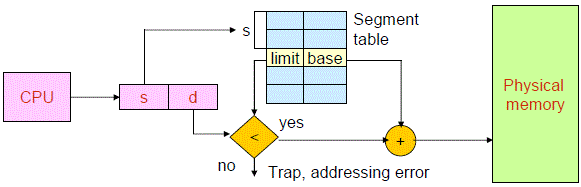
\includegraphics[scale=0.3]{images/segmentation.png}
  \end{figure}  
\end{frame}

\begin{frame}
  \frametitle{\textbf{Memoria Virtual} con Paginación}
  \begin{itemize}
  	\item La técnica de paginación intenta alocar la mayor cantidad de páginas necesarias posibles
	\item Cada vez que hay que alocar una página en un \emph{marco}, se produce un \textbf{fallo de página} (page fault) $\rightarrow$ \emph{hard page fault}
	\item ¿Qué sucede si es necesario alocar una página y ya no hay espacio disponible?
	\pause
	\item Se debe seleccionar una página víctima, para lo cual existen diversos algoritmos
	\item ¿Cuál es el mejor algoritmo?:
	\pause
	\begin{itemize}
		\item El que seleccione como página víctima aquella que no vaya a ser referenciada en un futuro próximo
	\end{itemize}
	\item La mayoria de los algoritmos predicen el comportamiento futuro mirando el comportamiento pasado
  \end{itemize}  
\end{frame}

\begin{frame}
  \frametitle{Algoritmo \textbf{Óptimo}}
  \begin{itemize}
  	\item Selecciona la página cuyo próxima referencia se encuentra más lejana a la actual
	\item Imposible de implementar $\rightarrow$ no se conoce los futuros eventos	  	
  \end{itemize}
  \begin{table}
	  \centering
	  \resizebox{\textwidth}{!}{
	  \begin{tabular}{| c | c | c | c | c | c | c | c | c | c | c | c |}
	      \hline
	      \bf Marco/Página & \bf 1 & \bf 2 & \bf 1 & \bf 3 & \bf 4 & \bf 1 & \bf 4 & \bf 3 & \bf 5 \\
	      \hline
	      \bf F1 & 1 & 1 & 1 & 1 & 1 & 1 & 1 & 1 & ? \\
	      \hline
	      \bf F2 &  & 2 & 2 & 2 & 4 & 4 & 4 & 4 & ? \\
	      \hline
	      \bf F3 &  &  &  & 3 & 3 & 3 & 3 & 3 & ? \\
	      \hline
	      \bf PF? & X & X &  & X & X &  &  &  & X \\
	      \hline
	  \end{tabular}
	  }
  \end{table}
  \textcolor{orange}{Continuación de la secuencia: 4 6 3 5 8 1}
\end{frame}

\begin{frame}
  \frametitle{Algoritmo \textbf{LRU}}
  \begin{itemize}
  	\item El algoritmo \emph{LRU} (Least Recently User) reemplaza la página que no fue referenciada por más tiempo
	\item Cada página debe tener información del instante de su última referencia $\rightarrow$ el overhead es mayor
  \end{itemize}
  \begin{table}
	  \centering
	  \resizebox{\textwidth}{!}{
	  \begin{tabular}{| c | c | c | c | c | c | c | c | c | c | c | c |}
	      \hline
	      \bf Marco/Página & \bf 1 & \bf 2 & \bf 1 & \bf 3 & \bf 4 & \bf 1 & \bf 4 & \bf 3 & \bf 5 \\
	      \hline
	      \bf F1 & 1 & 1 & 1 & 1 & 1 & 1 & 1 & 1 & 5 \\
	      \hline
	      \bf F2 &  & 2 & 2 & 2 & 4 & 4 & 4 & 4 & 4 \\
	      \hline
	      \bf F3 &  &  &  & 3 & 3 & 3 & 3 & 3 & 3 \\
	      \hline
	      \bf PF? & X & X &  & X & X &  &  &  & X \\
	      \hline
	  \end{tabular}
	  }
  \end{table}
\end{frame}

\begin{frame}
  \frametitle{Algoritmo \textbf{FIFO}}
  \begin{itemize}
  	\item El algoritmo \emph{FIFO} (Fist In First Out) trata a los \emph{frames} en uso como una cola circular
	\item Simple de implementar
	\item La página más vieja en la memoria es reemplazada
	\item La página puede ser necesitada pronto
  \end{itemize}
  \begin{table}
	  \centering
	  \resizebox{\textwidth}{!}{
	  \begin{tabular}{| c | c | c | c | c | c | c | c | c | c | c | c |}
	      \hline
	      \bf Marco/Página & \bf 1 & \bf 2 & \bf 1 & \bf 3 & \bf 4 & \bf 1 & \bf 4 & \bf 3 & \bf 5 \\
	      \hline
	      \bf F1 & 1 & 1 & 1 & 1 & 4 & 4 & 4 & 4 & 4 \\
	      \hline
	      \bf F2 &  & 2 & 2 & 2 & 2 & 1 & 1 & 1 & 1 \\
	      \hline
	      \bf F3 &  &  &  & 3 & 3 & 3 & 3 & 3 & 5 \\
	      \hline
	      \bf PF? & X & X &  & X & X & X &  &  & X \\
	      \hline
	  \end{tabular}
	  }
  \end{table}
\end{frame}

\begin{frame}
  \frametitle{Algoritmo \textbf{FIFO con segunda chande}}
  \begin{itemize}
  	\item Se utiliza un \emph{bit} adicional $\rightarrow$ bit de referencia
	\item Cuando la página se carga en memoria, el \emph{bit R} se pone a 0
	\item Cuando la página es referenciada el \emph{bit R} se pone en 1
	\item La víctima se busca en orden \emph{FIFO}. Se selecciona la primer página cuyo \emph{bit R} esta en 0
	\item Mientras se busca la víctima cada \emph{bit R} que tiene el valor 1, se cambia a 0
  \end{itemize}  
\end{frame}

\begin{frame}
  \frametitle{Algoritmo \textbf{FIFO}}
  \begin{itemize}
  	\item El algoritmo \emph{FIFO} (Fist In First Out) trata a los \emph{frames} en uso como una cola circular
	\item Simple de implementar
	\item La página más vieja en la memoria es reemplazada
	\item La página puede ser necesitada pronto
  \end{itemize}
  \begin{table}
	  \centering
	  \resizebox{\textwidth}{!}{
	  \begin{tabular}{| c | c | c | c | c | c | c | c | c | c | c | c |}
	      \hline
	      \bf Marco/Página & \bf 1 & \bf 2 & \bf 1 & \bf 3 & \bf 4 & \bf 1 & \bf 4 & \bf 3 & \bf 5 \\
	      \hline
	      \bf F1 & 1 & 1 & 1* & 1* & 1 & 1* & 1* & 1* & 1 \\
	      \hline
	      \bf F2 &  & 2 & 2 & 2 & 4 & 4 & 4* & 4* & 4 \\
	      \hline
	      \bf F3 &  &  &  & 3 & 3 & 3 & 3 & 3* & 5 \\
	      \hline
	      \bf PF? & X & X &  & X & X &  &  &  & X \\
	      \hline
	  \end{tabular}
	  }
  \end{table}
  \textcolor{orange}{* = \emph{bit R} = 1}
\end{frame}

\begin{frame}
  \frametitle{Paginación - Asignación de \emph{marco}}
  \begin{itemize}
  	\item La asignación de \emph{marco} se puede realizar de dos modos:
  	\begin{itemize}
  		\item \textbf{Asignación Fija}: a cada proceso se le asigna una cantidad arbitraria de \emph{marco}. A su vez para el reparto se puede usar:
  		\begin{itemize}
  			\item \textbf{Reparto equitativo}: se asigna la misma cantidad de \emph{marcos} a cada proceso $\rightarrow$ \textit{m div p}
  			\item \textbf{Reparto proporcional}: se asignan \emph{marco} en base a la necesidad que tiene cada proceso $\rightarrow$ \textit{V$_p$ . m / V$_t$}
  		\end{itemize}
		\item \textbf{Asignación dinámica}: los procesos se van cargando en forma dinámica de acuerdo a la cantidad de marcos que necesiten		
  	\end{itemize}
  \end{itemize}
\end{frame}

\begin{frame}
  \frametitle{Paginación - Alcance del reemplazo}
  \begin{itemize}
  	\item Al momento de seleccionar una página víctima, podemos utilizar:
  	\begin{itemize}
  		\item \textbf{Reemplazo global}: el fallo de página de un proceso puede reemplazar la página de cualquier proceso
		\item \textbf{Reemplazo local}: el fallo de página de un proceso solo puede reemplazar sus propias páginas
  	\end{itemize}
  \end{itemize}
\end{frame}

\begin{frame}
  \frametitle{Paginación - Descarga asincrónica de páginas}
  \begin{itemize}
  	\item El sistema operativo reserva uno o varios \emph{marco} para la descarga asincrónica de páginas
  	\item Cuando es necesario descargar una página modificada:
  	\begin{itemize}
  		\item La página que provoco el fallo se coloca en un \emph{frame} designado a la descarga asincrónica
		\item El SO envía la orden de descargar asincrónicamente la página modificada mientras continua la ejecución de otro proceso
		\item El \emph{frame} de descarga asincrónica pasa a ser el que contenía a la página víctima que ya se descargó correctamente
  	\end{itemize}
  \end{itemize}
\end{frame}

\begin{frame}
  \frametitle{Descarga asincrónica de páginas (ejemplo)}
  \begin{itemize}
  	\item \textcolor{orange}{Ejemplo de algoritmo \emph{FIFO}}
	\begin{figure}
	    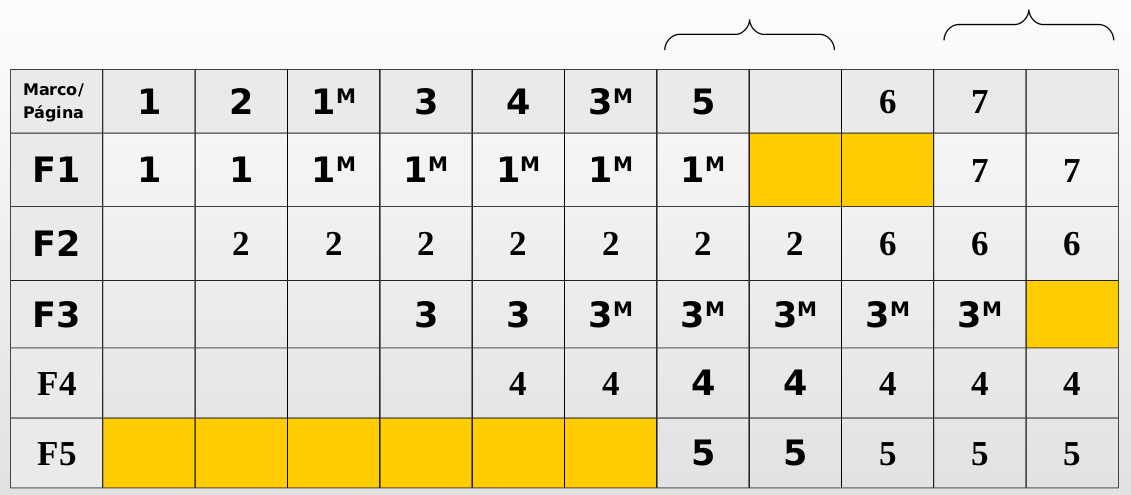
\includegraphics[scale=0.2]{images/asyncDownload.png}
	\end{figure}  	
  \end{itemize}
\end{frame}

\begin{frame}
  \frametitle{Paginación - \textbf{Performance}}
  \begin{itemize}
  	\item La técnica de paginación por demanda puede generar una degradación de rendimiento del sistema debido a que el reemplazo de páginas es costoso
  	\item Tasa de \emph{page faults 0 $\langle$ p $\langle$ 1}:
  	\begin{itemize}
  		\item Si \emph{p = 0}, no hay \emph{page faults}
		\item Si \emph{p = 1}, cada referencia es un \emph{page fault}
  	\end{itemize}
  	\item \emph{Effective Access Time}: medida utilizada para medir este costo:
  	\begin{itemize}
  		\item \textbf{Am} = tiempo de acceso a la memoria real
  		\item \textbf{Tf} = tiempo de atención de un fallo de página
  		\item \textbf{At} = tiempo de acceso a la tabla de páginas. Es igual al tiempo de acceso a la memoria (\emph{Am}) si la entrada de la tabla de páginas no se encuentra en la \emph{TLB} (cache donde residen las traducciones de direcciones realizadas)
  	\end{itemize}
  	\hspace{35pt} \textbf{TAE = At + ( 1 - p ) * Am + p * ( Tf + Am )}
  \end{itemize}
\end{frame}

\begin{frame}
  \frametitle{\textbf{Thrashing}}
  \begin{itemize}
  	\item \emph{Thrashing} (hiperpaginación):
  	\begin{itemize}
  		\item decimos que un sistema está en \emph{thrashing} cuando pasa más tiempo paginando que ejecutando procesos
  	\end{itemize}
  	\item Si un proceso cuenta con todos los \emph{frames} que necesita, no habría \emph{thrashing}. Salvo excepciones como la \emph{anomalía de \textbf{Belady}}
  	\item Existen técnicas para evitarlo $\rightarrow$ estrategia de \emph{Working Set}
  \end{itemize}
\end{frame}

\begin{frame}
  \frametitle{Working Set - \textbf{Modelo de Localidad}}
  \begin{itemize}
  	\item Las referencias a datos y programas dentro de un proceso tienden a agruparse
  	\item La localidad de un proceso en un momento dado se da por el conjunto de páginas que son referenciadas en ese momento
  	\item En cortos períodos de tiempo, el proceso necesitará pocas ``piezas'' del proceso (una página de instrucciones y otra de datos)
  	\item Entonces se define una ventana de trabajo o \emph{working set} ($\Delta$) que contiene las referencias de memoria más recientes
  	\item \textbf{Working Set}: es el conjunto de páginas que tienen las $\Delta$ referencias a páginas más recientes
  \end{itemize}
\end{frame}

\begin{frame}
  \frametitle{Selección del $\Delta$}
  \begin{itemize}
    \item $\Delta$ chico: no cubrirá la localidad. Toma muy pocas referencias
    \item $\Delta$ grande: puede tomar varias localidades. Toma referencias de la localidad y algunas más, posiblemente viejas
    \item Para determinar la medida del \emph{working set} debemos tener en cuenta:
    \begin{itemize}
      \item \emph{m} = cantidad de \emph{frames} disponibles
      \item \emph{D} = demanda total de \emph{frames}
      \item \emph{WSS$_i$} = medida del \emph{working set} del proceso$_i$
      \item \emph{$\sum$ WSS$_i$} = \emph{D}
      \item Si \emph{D $\rangle$ m} habrá \textbf{thrashing}
    \end{itemize}    
  \end{itemize}
\end{frame}